\subsection{Materiali e circuiti}

Per costruire i due circuiti in esame, mostrati in Figura \ref{fig:circuits},
abbiamo utilizzato i seguenti materiali:

\begin{itemize}
    \item{Breadboard, cavi a banana e cavetti da breadboard.}
    \item{Amplificatore operazionale LM741.}
    \item{Resistenze: \SI{3.9}{\kilo\ohm}, \SI{50}{\kilo\ohm}, \SI{100}{\kilo\ohm}
        e una variabile per simulare un carico con impedenza non costante. Nel nostro caso abbiamo
        usato una resistemza con un range operativo da 0 a \SI{10}{\kilo\ohm}.}
    \item{Alimentatore di corrente continua.}
    \item{Generatore di funzioni d'onda Agilent 33120A.}
    \item{Multimetro Agilent 34410A.}
    \item{Oscilloscopio Agilent DSO-X 2002A, con generatore di funzioni d'onda integrato
        (purtroppo questo modello ha solo 2 canali di input,
        per il test del sommatore sarebbe stato meglio avere un oscilloscopio con almeno 3 input).}
\end{itemize}

\begin{figure}[h]
        \centering
        \begin{subfigure}[b]{0.48\textwidth}
                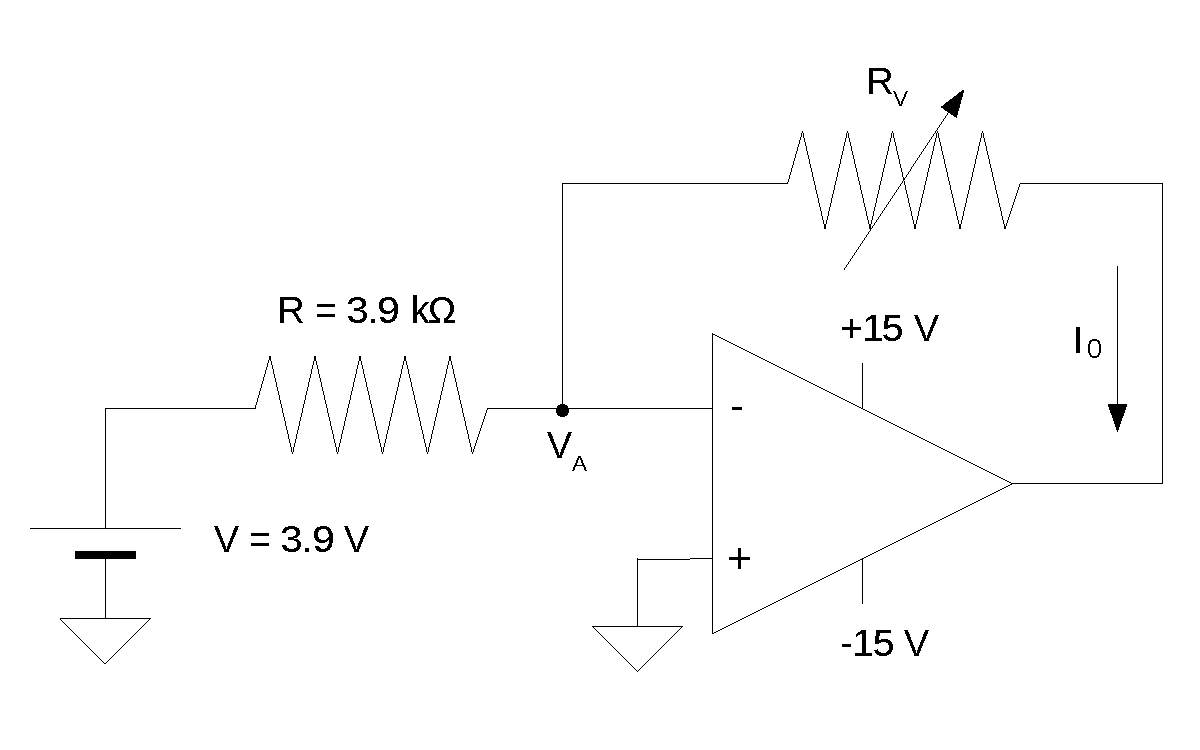
\includegraphics[width=\textwidth]{figure/schema_gen_corr.pdf}
                \caption{Generatore di corrente costante}
                \label{fig:generatore}
        \end{subfigure}
        ~
        \begin{subfigure}[b]{0.48\textwidth}
                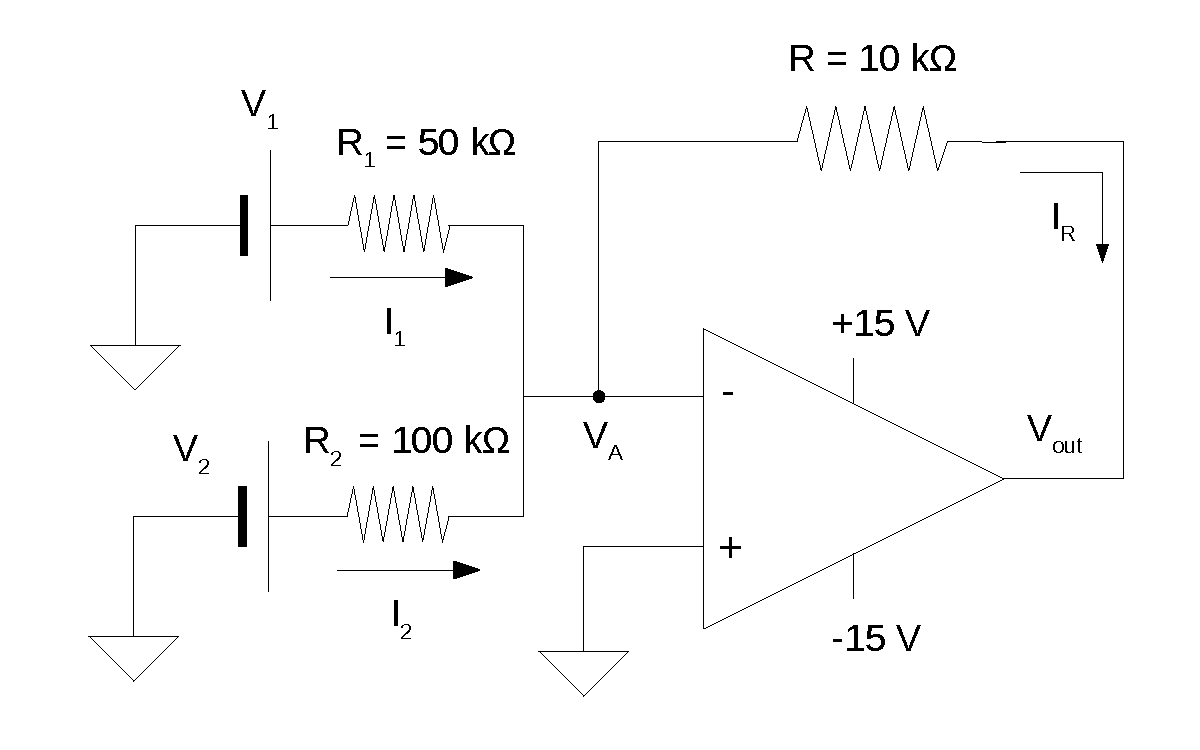
\includegraphics[width=\textwidth]{figure/circuito_sommatore.pdf}
                \caption{Sommatore pesato di tensioni}
                \label{fig:sommatore}
        \end{subfigure}
        \caption{Circuiti costruiti durante l'esperienza}
        \label{fig:circuits}
\end{figure}

